%\documentclass[10pt]{article}
%\usepackage[utf8]{inputenc}
%\usepackage[T1]{fontenc}
%\usepackage{amsfonts}
%\usepackage{amssymb}
%\usepackage{geometry}
%\usepackage{pstricks,pst-eucl}
%\usepackage{tikz}
%\usepackage{graphics}
%\usepackage{pslatex}
%\usepackage{lscape}
%\usepackage{eurosym}
%\usepackage{skak}
%\usepackage{chessboard}

\documentclass[11pt, a4paper]{report}
%\documentclass[11pt, a4paper]{article}

%====================== PACKAGES ======================

\usepackage[french]{babel}
\frenchbsetup{StandardLists=true}
\usepackage{enumitem}
\usepackage{pifont}
\usepackage[utf8x]{inputenc}
\usepackage[T1]{fontenc}
%pour gérer les positionnement d'images
\usepackage{float}
\usepackage{amsmath}
\DeclareMathOperator{\dt}{dt}
\usepackage{graphicx}
\usepackage{tabularx}
\usepackage[colorinlistoftodos]{todonotes}
\usepackage{url}
%pour les informations sur un document compilé en PDF et les liens externes / internes
\usepackage[pdfborder=0]{hyperref}
\hypersetup{
	colorlinks = true
	}
%pour la mise en page des tableaux
\usepackage{array}
\usepackage{tabularx}
\usepackage{multirow}
\usepackage{multicol}
\setlength{\columnsep}{50pt}
%espacement entre les lignes
\usepackage{setspace}
%modifier la mise en page de l'abstract
\usepackage{abstract}
%police et mise en page (marges) du document
\usepackage[T1]{fontenc}
\usepackage[top=2cm, bottom=2cm, left=2cm, right=2cm]{geometry}
%Pour les galerie d'images
\usepackage{subfig}

\usepackage{pdfpages}
%\usepackage{tikz}

\usepackage{appendix}

\usepackage{comment}

\usepackage{skak}
\usepackage{chessboard}

%\usetikzlibrary{angles, quotes}
%\usetikzlibrary{decorations.pathmorphing}
%====================== INFORMATION ET REGLES ======================

%rajouter les numérotation pour les \paragraphe et \subparagraphe
\setcounter{secnumdepth}{4}
\setcounter{tocdepth}{4}

\hypersetup{							% Information sur le document
pdfauthor = {Stephan Runigo},			% Auteurs
pdftitle = {Recueil d'echec},			% Titre du document
pdfsubject = {Répertoire d'ouverture et parties},		% Sujet
pdfkeywords = {échec, ouverture},	% Mots-clefs
pdfstartview={FitH}}	% ajuste la page à la largeur de l'écran
%pdfcreator = {MikTeX},% Logiciel qui a crée le document
%pdfproducer = {} % Société avec produit le logiciel
%======================== DEBUT DU DOCUMENT ========================
%
\begin{document}
%
%régler l'espacement entre les lignes
\newcommand{\HRule}{\rule{\linewidth}{0.5mm}}
%
%page de garde	%
%\begin{titlepage}
%
~\\[1cm]

\begin{center}
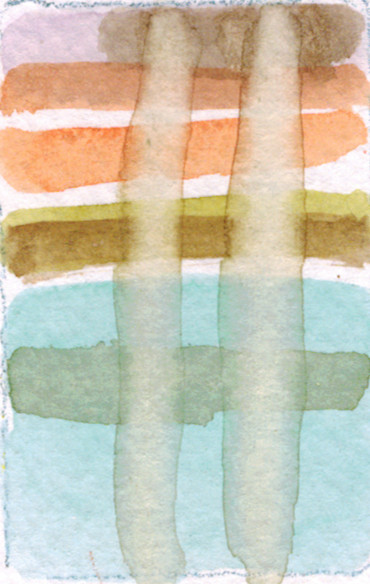
\includegraphics[scale=2]{./presentation/champ06}
\end{center}

\textsc{\Large }\\[0.5cm]

% Title \\[0.4cm]
\HRule

\begin{center}
{\huge \bfseries  Principes élémentaires\\
du jeu d'échec\\[0.4cm] }
\end{center}

\HRule \\[1.5cm]

\begin{center}
%\includegraphics[scale=0.3]{./presentation/ptoleme}
\end{center}

\begin{center}
%\includegraphics[scale=0.3]{./presentation/diagrammesInteractions}
\end{center}


% Author and supervisor
\begin{minipage}{0.4\textwidth}
\begin{flushleft} \large
\emph{Auteur:}\\
Stephan \textsc{Runigo}
\end{flushleft}
\end{minipage}
\begin{minipage}{0.4\textwidth}
\begin{flushright} \large
\emph{Illustration:}\\
Krikri
\end{flushright}
\end{minipage}

\vfill

% Bottom of the page
{\large \today}

\end{titlepage}

%
%page blanche	%
%\begin{center}
\Large
Résumé
\normalsize
\end{center}
\vspace{3cm}
\begin{itemize}[leftmargin=1cm, label=\ding{32}, itemsep=21pt]
\item {\bf Objet : Les ouvertures} .
\item {\bf Contenu : Principes élémentaires} .
\item {\bf Public concerné : Débutant} .
\end{itemize}

\vspace{3cm}



\vspace{3cm}


%\newpage
%~
%ne pas numéroter cette page
%\thispagestyle{empty}
	%\newpage

\tableofcontents
\thispagestyle{empty}
\setcounter{page}{0}
%ne pas numéroter le sommaire
%
%\newpage
%
%espacement entre les lignes d'un tableau
\renewcommand{\arraystretch}{1.5}
%
%====================== INCLUSION DES PARTIES ======================
%
~
\thispagestyle{empty}
%recommencer la numérotation des pages à "1"
\setcounter{page}{0}
\newpage
%	%
%
%
\newpage
%
\chapter{Ouvertures}

Ce chapitre traite des ouvertures.



%\input{./utilisation/exemple.tex}

\section{Principes élémentaires}
%
%%%%%%%%%%%%%%%%%%%%%
\subsection{Prendre le centre}
%%%%%%%%%%%%%%%%%%%%%
%
L'occupation du centre consiste à placer une pièce au centre. Cela peut être un pion ou une pièce mineure. Contrôler le centre consiste à placer une pièce qui attaque une ou plusieurs case du centre.

\begin{center}
\newgame
\mainline{1. e4 }
\def\empharea{ e4-e4 }
\chessboard[color=red,
	markstyle=color,markfields=d5,
	emphstyle=\color{green},
	empharea=\empharea]
\end{center}

Le pion e4 occupe une case centrale et contrôle la case centrale (d5). C'est un bon coup.

\begin{center}
\newgame
\mainline{1. Nf3 }
\def\empharea{ f3-f3 }
\chessboard[color=red,
	markstyle=color,markfields=d4,
	markstyle=color,markfields=e5,
	emphstyle=\color{green},
	empharea=\empharea]
\end{center}

Le cavalier f3 contrôle les deux cases centrales d4 et e5.

\newgame

\mainline{1. e4 e5 2. Nf3 Nc6}

\begin{center}
\chessboard
\end{center}

%\newchessgame
\newgame

\def\empharea{ h8-f4 }
\chessboard[emphstyle=\color{red},
empharea=\empharea]



%%%%%%%%%%%%%%%%%%%%%
\subsection{Se développer}
%%%%%%%%%%%%%%%%%%%%%
%

\subsubsection{Sortir les pièces mineures}


\subsubsection{Gagner du temps}

Créer une menace en se développant oblige l'adversaire à contrer cette menace. 



%%%%%%%%%%%%%%%%%%%%%
\subsection{Roquer}
%%%%%%%%%%%%%%%%%%%%%
%

%%%%%%%%%%%%%%%%%%%%%%%%%%%%%%%%%%%%%%%%%%%%%%%%%%%%%%%%%%%%%%%%%%%%%%%%


%%%%%%%%%%%%%%%%%%%%%%%%%%%%%%%%%%%%%%%%%%%%%%%%%%%%%%%%%%%%%%%%%%%%%%%%

%%%%%%%%%%%%%%%%%%%%%%%%%%%%%%%%%%%%%%%%%%%%%%%%%%%%%%%%%%
%
\section{Jouer l'écossaise}
%
%%%%%%%%%%%%%%%%%%%%%%%%%%%%%%%%%%%%%%%%%%%%%%%%%%%%%%%%%%
%
%L'écossaise se caractérise par le coup \texttt{3. d4} après les coups classiques \texttt{1. e4 e5 2. Cf3 Cc6} :
Après les coups classiques, fréquement joués
\newgame

\mainline{1. e4 e5 2. Nf3 Nc6}

\begin{center}
\chessboard
\end{center}


L'écossaise se caractérise par le coup
%les blancs rentre généralement dans la partie espagnole ou la partie italienne. Il peuvent également rentré dans la partie écossaise
%\textit{Projet Cavalier e5, Tour e1}
\mainline{3. d4}

%\textit{Fréquent : }\textit{}
%\variation{4. e5}


%\mainline{4... Bg4}

\begin{center}
\chessboard
\end{center}












\newgame

\mainline{1. e4 e6 2. d4 d5 3. e5}

\begin{center}
\chessboard
\end{center}


\newgame

\textit{Projet Cavalier e5, Tour e1}
\mainline{1. e4 e6 2. d4 d5 3. pxd5}

\begin{center}
\chessboard
\end{center}


\newgame
%rnbqkbnr/pppppppp/8/8/8/8/PPPPPPPP/RNBQKBNR

\begin{center}
\chessboard{rnbqkbnr/pppppppp/8/8/8/8/PPPPPPPP/RNBQKBNR w KQkq - 0 1}
\end{center}



%\mainline{3. exd}
%%%%%%%%%%%%%%%%%%%%%%%%%%%%%%%%%%%%%%%%%%%%%%%%%%%%%%%%%

%%%%%%%%%%%%%%%%%%%%%%%%%%%%%%%%%%%%%%%%%%%%%%%%%%%%%%%%%%
%
\section{Jouer contre la Française}
%
%%%%%%%%%%%%%%%%%%%%%%%%%%%%%%%%%%%%%%%%%%%%%%%%%%%%%%%%%%
%
\newgame

\mainline{1. e4 e6 2. d4 d5}

\begin{center}
\chessboard
\end{center}

\textit{Projet Cavalier e5, Tour e1}
\mainline{3. pexd5 pexd5}

\textit{Fréquent : }
%\variation{4. e5}


%\mainline{4... Bg4}

\begin{center}
\chessboard
\end{center}

\newgame

\mainline{1. e4 e6 2. d4 d5 3. e5}

\begin{center}
\chessboard
\end{center}


\newgame

\textit{Projet Cavalier e5, Tour e1}
\mainline{1. e4 e6 2. d4 d5 3. pxd5}

\begin{center}
\chessboard
\end{center}


\newgame
%rnbqkbnr/pppppppp/8/8/8/8/PPPPPPPP/RNBQKBNR

\begin{center}
\chessboard{rnbqkbnr/pppppppp/8/8/8/8/PPPPPPPP/RNBQKBNR w KQkq - 0 1}
\end{center}



%\mainline{3. exd}
%%%%%%%%%%%%%%%%%%%%%%%%%%%%%%%%%%%%%%%%%%%%%%%%%%%%%%%%%

%%%%%%%%%%%%%%%%%%%%%%%%%%%%%%%%%%%%%%%%%%%%%%%%%%%%%%%%%%%
%
\section{Les ouvertures de MVL}
%
%%%%%%%%%%%%%%%%%%%%%%%%%%%%%%%%%%%%%%%%%%%%%%%%%%%%%%%%%%
%
%
% D'après la vidéo
%  MVL contre Nepo - le match des marlous.mp4
%
\newgame

\subsection{Réfutation de 1. g3}

\mainline{1. g3 h5 2. Bg2 h4}

\begin{center}
\chessboard
\end{center}

\mainline{3. d4 d5 4. c4 e6}

\mainline{5. Nc3 c6 }
 %\mainline{6. e4 dc4}

%\textit{Fréquent : }
%\variation{4. e5}

\begin{center}
\chessboard
\end{center}

%rnbqkbnr/pppppppp/8/8/8/8/PPPPPPPP/RNBQKBNR

\begin{center}
%\chessboard{rnbqkbnr/pppppppp/8/8/8/8/PPPPPPPP/RNBQKBNR w KQkq - 0 1}
\end{center}



%\mainline{3. exd}
%%%%%%%%%%%%%%%%%%%%%%%%%%%%%%%%%%%%%%%%%%%%%%%%%%%%%%%%%

%\input{./ouverture/.tex}

%

%
%
%====================== INCLUSION DE LA BIBLIOGRAPHIE ======================
%
%récupérer les citation avec "/footnotemark"
%\nocite{*}
%choix du style de la biblio
\bibliographystyle{plain}
%inclusion de la biblio
\cleardoublepage
\addcontentsline{toc}{chapter}{Bibliographie}
\bibliography{bibliographie.bib}
%\newpage
%\input{./glossaire/glossaire.tex}
%\newpage
%\input{./annexes/annexes.tex}
\end{document}
%%%%%%%%%%%%%%%%%%%%%%%%%%%%%%%%%%%%%%%%%%%%%%%%%%%%%%%%%%%%%%%%%%%%%%%%%%%%%%%%%
